\documentclass[11pt,a4paper]{article}

\usepackage[utf8]{inputenc}
\usepackage[spanish,mexico]{babel}

\usepackage{amsmath, amssymb, amsthm}
%\usepackage{mathrsfs}
\usepackage{appendix}
%\usepackage{minted}	

%pdflatex -synctex=1 -interaction=nonstopmode --shell-escape %.tex


\usepackage{hyperref}
\usepackage{captdef}

\usepackage{psfrag}
\usepackage{graphicx}
%\usepackage{subfig}
\usepackage{color}
\usepackage{multicol} 
\usepackage{wrapfig}

%\usepackage{fancyhdr}
%\pagestyle{fancy}
%\fancyhf{}


\usepackage{cancel}
\usepackage[usenames,dvipsnames,svgnames,table]{xcolor}
\usepackage[left=2cm,right=2cm,top=2cm,bottom=2cm]{geometry}
\usepackage{caption}
\usepackage{subcaption}
%\renewcommand{\baselinestretch}{1.5}

\usepackage{hyperref}
%\usepackage[hidelinks]{hyperref} 
\hypersetup{
	colorlinks=true,
	linkcolor=blue,
	filecolor=magenta,      
	urlcolor=cyan,
}

\begin{document}
\thispagestyle{empty}

\includegraphics[height=3.5cm]{escudoCiencias.pdf}
\vspace{-3.8cm}
\begin{flushright}
	\hspace{4cm}
	{\Large\textbf{Sobre los Métodos.}\\
		Proyecto de Tesis}
	\vspace{0.3cm}\\
	\begin{large}Autor: Rodrigo Vega Vilchis.\end{large}\\
	\begin{footnotesize}
		Correo: rockdrigo6@ciencias.unam.mx\\
		\hspace{2.05cm}{\color{white}.}\\
	\end{footnotesize}
	\vspace{0.1cm}
	\begin{large}
		Fecha: 19 Agosto, 2024\end{large}\\
\end{flushright}
%\vspace{.4cm}
\hrule height1pt\vspace{.5cm}

\begin{abstract}
	hola
\end{abstract} 
	
\section{Explicaciones técnicas}

\subsection{Sistema de competencia de especies para $n=2$}

El sistema de Lotka-Volterra es uno de los sistemas utilizados para poder comprender la naturaleza de la dinámica no lineal. En este caso particular, los términos no lineales son cuadráticos y representan la interacción entre la especie $i$ y la especie $j$. 
\begin{equation}\label{eqn:LK}
	\frac{dx_i}{dt}=r_ix_i\left(1-\frac{\sum_{j=1}^N \alpha_{ij}x_j}{K_i}\right)
\end{equation}
Se considera una tasa de crecimiento $r_i$ para la especie $i$, una capacidad de carga $K_i$ que limita hasta cierto punto su crecimiento, y su respectiva interacción con la especie $x_j$ cuya ``fuerza'' de interacción esta dada por los coeficientes $\alpha_{ij}$. Al ser un sistema de ecuaciones diferenciales no lineales, no es posible acceder a una solución analítica general\footnote{debido a los términos no lineales... (me gustaría una explicación más completa: ver strogatz y tratados de ecuaciones diferenciales).}; por ello se recurre a métodos de integración numérica capaces de aproximar las soluciones a un rango considerable y cercano a la solución real. El método empleado por excelencia en este trabajo es el integrador Runge-Kutta de orden 4\footnote{poner una referencia de libro}.\\
\\
De manera pedagógica para aprender y analizar las virtudes y comportamientos del sistema \ref{eqn:LK} es recomendable comenzar por explorar el sistema de $2\times 2$.
$$
\begin{cases}
	\dot{x}_1&=r_1x_1(1-\frac{a_{11}x_1}{k_1}-\frac{a_{12}x_1x_2}{k_1})\\
	\dot{x}_2&=r_2x_2(1-\frac{a_{21}x_1x_2}{k_2}-\frac{a_{22}x_2}{k_2})
\end{cases}
$$
En este caso particular, tenemos una tasa de crecimiento y una capacidad de carga personalizada para cada especie, lo que es razonable con el hecho de que cada especie crece a un ritmo determinado y también es limitada de manera determinada. En este caso los coeficientes $\alpha_{ij}$ forman parte de una matriz de \textit{incidencias} entre especies definida de la siguiente manera
\begin{equation}\label{eqn:mIncidencias}
	A=
	\begin{pmatrix}
		1 & \alpha_{12}\\
		\alpha_{21} &1
	\end{pmatrix}
\end{equation}
Es apreciable que los términos de la diagonal se encuentran en $\alpha_{ii} = 1$\footnote{Argumentar más adelante.} respectivamente, más adelante se dará una explicación detallada de esta característica; por el momento solo nos enfocaremos en la dinámica que produce el sistema. Para ello se define el siguiente sistema
\begin{align*}
	\frac{dx}{dt}&=2x\left(1-\frac{x}{2}\right)-xy\\
	\frac{dy}{dt}&=3y\left(1-\frac{y}{3}\right)-2xy
\end{align*}
De este sistema se pueden notar algunas características: se tiene para cada ecuación diferencial (especie) una tasa de crecimiento y una capacidad de carga específica o personalizada. Por ejemplo para la ecuación $\dot{x}$ se tiene una tasa de crecimiento y capacidad de carga de 2 para la especie $x$ y para la especie $y$ estos valores son iguales a 1; para la ecuación $\dot{y}$ se tiene una tasa de crecimiento y capacidad de carga de 3 para la especie $x$ y para la especie $y$ se tiene una tasa de crecimiento de 2 y una capacidad de carga de 1. Aunque este sistema tal cual no tiene una solución analítica per se, si es posible explorar acerca de su comportamiento; en principio se pueden hallar sus puntos fijos que nos hablan de la estabilidad del sistema. Para hallar puntos fijos es necesario encontrar las raíces de este sistema. La solución trivial siempre será $(0,0)$, de ahí se tienen que igualar a cero las ecuaciones para hallar los otros puntos críticos.
\begin{align*}
	2x-x^2-xy &= 0,\qquad\text{suponiendo que $y = 0$}\\
	2x &= x^2\\
	x&=2
\end{align*}
y para $\dot{y}$ se tiene
\begin{align*}
	3y-y^2-2xy&=0,\qquad\text{suponiendo que $x=0$}\\
	3y &= y^2\\
	y &= 3
\end{align*}
Por tanto tenemos para $\dot{x}$ el punto fijo $(2,0)$ mientras que para $\dot{y}$ se tiene el punto fijo $(0,3)$. Aún es posible hallar un último punto fijo que es para cuando ambas ecuaciones se hacen cero.
\begin{align*}
	2x-x^2-xy&=0,\qquad\text{Se despeja $y$ de esta ecuación.}\\
	xy &= x(2-x)\\
	y &= (2-x)\\
	\\
	3(x-2)-(x-2)^2-2x(x-2) &= 0\\
	3x-6-(x^2-4x+4)-2x^2+4x&=0,\qquad\text{Reduciendo términos se tiene.}\\
	x^2-3x+2 &= 0
\end{align*}
%%%%%%%%%%%%%%%%%%%%%CHECKPOINT
Al resolver esta última ecuación se determina el último punto fijo que corresponde a $(1,1)$. Los puntos fijos brindan información para explorar hacia donde pueden converger (atractores) o diverger (repulsores o puntos sillas) las soluciones del sistema dependiendo de las condiciones iniciales que se le impongan.\footnote{explicar brevemente de que se trata uno, quizás esto deba precisarse desde la introducción.} Se establece que si las soluciones convergen entonces el sistema es considerado \textit{estable} mientras que 
\begin{wrapfigure}{r}{0.5 \textwidth} \vspace{-30pt} \begin{center}
		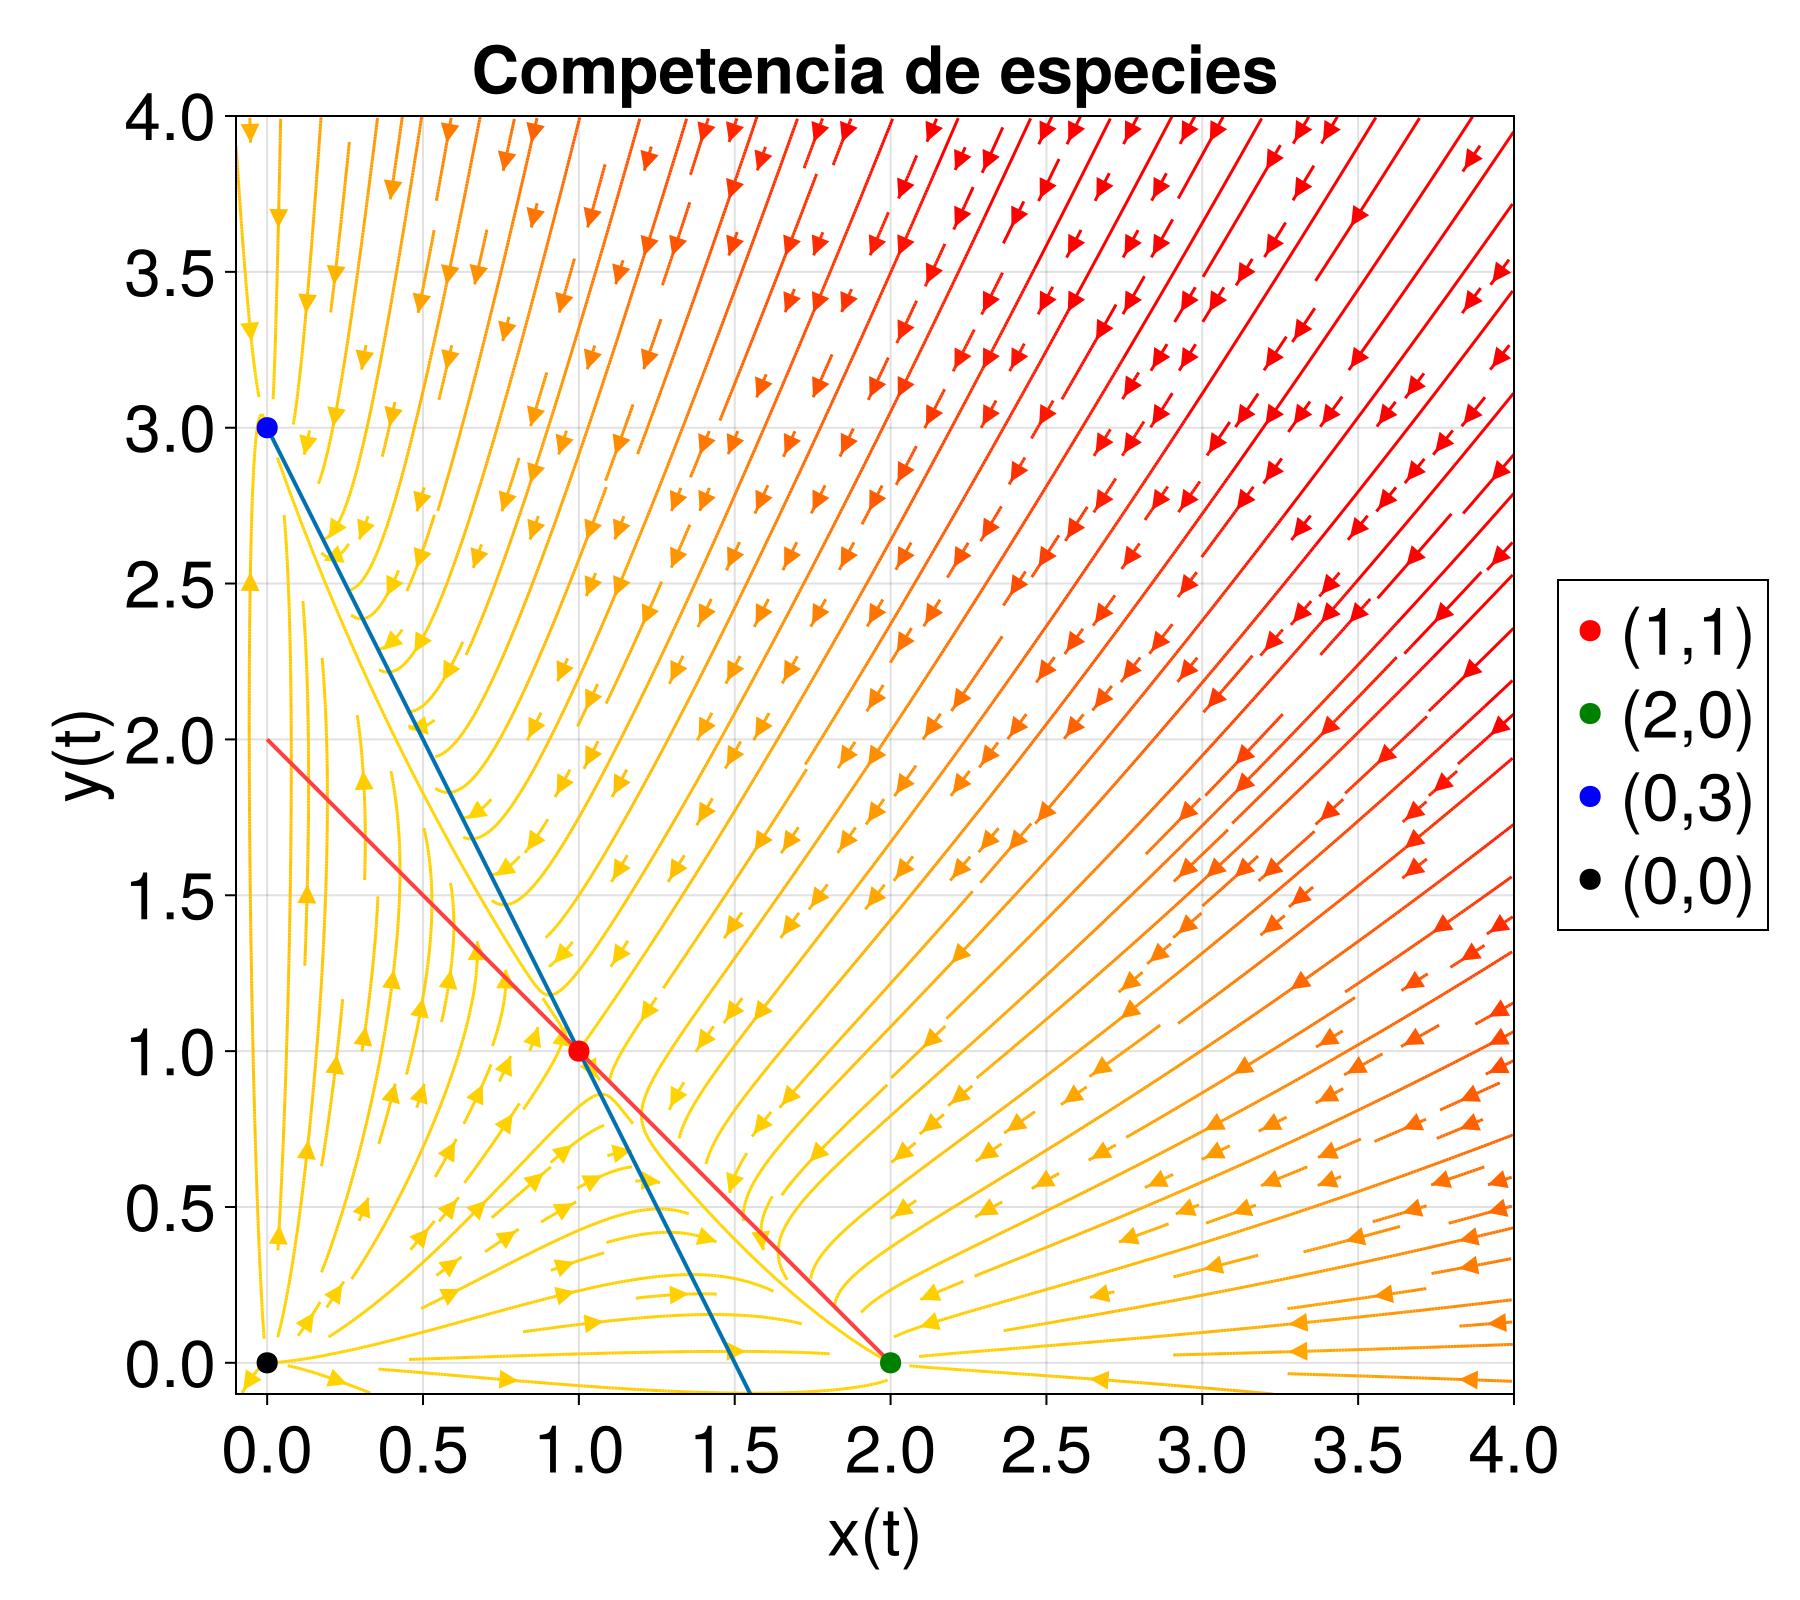
\includegraphics[width=0.45\textwidth]{../Imagenes/Competencia de especies} 
		\end{center} 
		\vspace{-20pt} 
		\caption{Campo vectorial de las soluciones del sistema propuesto.} 
		\vspace{-10pt}
		\label{fig:CompetenciaEspecies}
\end{wrapfigure} 
en caso contrario el sistema es considerado \textit{inestable.} Es posible determinar mediante técnicas computacionales el campo vectorial de las soluciones de este sistema\footnote{Realizar referencia de la técnica empleada.}, inclusive dos de las isoclinas\footnote{si son isoclinas???} del sistema resolviendo las ecuaciones igualando a cero y despejando $y$ de cada una de ellas. Es notorio como dichas isoclinas inciden de alguna forma en tres de los puntos fijos. El gráfico nos muestra que las soluciones convergen hacia los puntos que se encuentran en los ejes; todo dependerá de las condiciones iniciales del sistema para ver hacia donde convergen. El punto fijo de en medio es conocido como punto silla y es inestable ya que aunque existan soluciones que convergan hacia él mismo, en la mínima perturbación que se le provoque la solución puede ``desviarse'' hacia los atractores. Por último se observa que del origen divergen todas las soluciones por lo que es considerado un punto fijo repulsor.\\
\\
%%%%%%%%%%%%%%%%%%%%%CHECKPOINT
%% Nada más checar la aseveración de las isoclinas para ver si se queda o se retira del párrafo
En esta ocasión por tratarse de un sistema de $2\times 2$, se tuvo la fortuna de poder obtener una representación visual del sistema y poder realizar un análisis cualitativo del mismo para sacar conclusiones. Pero ¿qué sucede cuando se tienen sistemas de $N$ especies? En principio el espacio vectorial (fase) de las soluciones se vuelve $N-$dimensional y por lo tanto imposible de visualizar en un gráfico. Es por ello que se requieren de otras técnicas analíticas para seguir esbozando el comportamiento del sistema. Una herramienta útil a esta conjetura es la de \textit{linealizar}\footnote{Explicar brevemente en esta nota a que se refiere esto.} el sistema para poder explorar el comportamiento de los puntos fijos a nivel local. Para realizar esta acción es necesario aplicar el \textit{Jacobiano} al sistema para ``bajar'' el grado de las ecuaciones del sistema \ref{eqn:LK} y así obtener puras ecuaciones lineales.\\
\\
Se define la función vectorial $\mathbf{F}:\mathbb{R}^n\to\mathbb{R}^n$, donde $n$ será el número de especies del sistema de Lotka-Volterra generalizado \ref{eqn:LK}.
\begin{equation}\label{eqn:LKmatricial}
	\mathbf{F}(\vec{x})=\begin{pmatrix}
		f_1(\vec{x})=\dot{x}_1\\
		\vdots\\
		f_n(\vec{x}))=\dot{x}_n
	\end{pmatrix},\qquad\text{donde $\vec{x}=\left(x_1(t),...,x_n(t))\right)$.}
\end{equation}
Las componentes de $\mathbf{F}(\vec{x})$ corresponden con las funciones del sistema \ref{eqn:LK}, y las componentes del vector $\vec{x}$ corresponden con sus especies involucradas. Por tanto el Jacobiano del sistema quedaría de la siguiente forma
\begin{equation}\label{eqn:Jacobiano}
	\mathbb{J}_\mathbf{F}(\vec{x}) = \begin{pmatrix}
		\frac{\partial f_1(\vec{x})}{\partial x_1} & \cdots &\frac{\partial f_1(\vec{x})}{\partial x_n}\\
		\vdots & \ddots & \vdots\\
		\frac{\partial f_n(\vec{x})}{\partial x_1} & \cdots &\frac{\partial f_n(\vec{x})}{\partial x_n}
	\end{pmatrix}
\end{equation}
Esta resultante al ser evaluada en los puntos fijos del sistema genera la llamada matriz de \textit{interacciones} que es aquella que nos brinda la información necesaria para determinar la estabilidad de ese punto fijo en particular. Por ello se establece que la matriz de interacciones brinda información solo a nivel local, pues no contiene información de otros puntos fijos ajenos. Para validar esta aseveración ocuparemos nuestro sistema de $2\times 2$ y relacionaremos la matriz de interacciones con lo que se muestra en el gráfico. El Jacobiano del sistema \ref{eqn:LK} para $n=2$ es el siguiente
\begin{equation}\label{eqn:Jacobiano2}
	\mathbb{J}_\mathbf{F}(\vec{x})=\begin{pmatrix}
		r_1-\frac{2r_1x_1+r_1a_{12}x_2}{K_1} & -\frac{r_1a_{12}x_1}{K_1}\\
		-\frac{r_2a_{21}x_2}{K_2} & r_2-\frac{2r_2x_2+r_2a_{21}x_1}{K_2}
	\end{pmatrix}
\end{equation}
debido a la matriz de incidencias \ref{eqn:mIncidencias}, se tiene que los valores $a_{ii}=1$ que corresponden con las auto-interacciones. Evaluando los puntos fijos antes encontrados en el jacobiano \ref{eqn:Jacobiano2} se tienen las siguientes matrices de interacciones:
$$
\mathbb{J}_{(2,0)} = \begin{pmatrix}
	-2 & -2\\
	0 & -1
\end{pmatrix},\qquad \mathbb{J}_{(0,3)}=\begin{pmatrix}
-1 & 0\\
-6 & -3
\end{pmatrix},\qquad \mathbb{J}_{(1,1)}=\begin{pmatrix}
-1 & -1\\
-2 & -1
\end{pmatrix},\qquad \mathbb{J}_{(0,0)}=\begin{pmatrix}
2 & 0 \\
0 & 3
\end{pmatrix}
$$
%%%%%%%%Checkpoint
Como previamente se ha revisado\footnote{Hay que referenciar este enunciado con algún sustento de la introducción en donde se maneje el tema de los eigenvalores y eigenvectores como solución de sistemas lineales.}, los eigenvalores (más que los eigenvectores) determinan la estabilidad de un sistema lineal. Se establece que mientras ellos tengan parte real negativa se asegurará que el sistema será estable y que en otro caso el sistema será inestable. Por lo tanto los eigenvalores de las primeras dos matrices de interacciones deben ser negativos para que sustenten los atractores de la figura \ref{fig:CompetenciaEspecies}. Mientras que los eigenvalores de $\mathbb{J}_{(1,1)}$ deben ser uno negativo y otro positivo para sustentar al punto silla. Para la matriz $\mathbb{J}_{(0,0)}$ sus eigenvalores deben ser positivos para que sustenten el repulsor. Realizando el álgebra correspondiente se encuentra lo siguiente
\begin{align*}
	\mathbb{J}_{(2,0)}&\Longrightarrow\ \lambda_1 = -2,\quad\lambda_2 = -1\\
	\mathbb{J}_{(0,3)}&\Longrightarrow\ \lambda_1 = -3,\quad\lambda_2 = -1\\
	\mathbb{J}_{(1,1)}&\Longrightarrow\ \lambda_1 = -1+\sqrt{2},\quad\lambda_2 = -1-\sqrt{2}\\
	\mathbb{J}_{(0,0)}&\Longrightarrow\ \lambda_1 = 2,\quad\lambda_2 = 3\\
\end{align*}
Por tanto se termina de validar la consistencia del método de la linearización para esbozar la estabilidad de \ref{eqn:LK} por cada uno de sus puntos fijos. Esta forma analítica de reconocer la estabilidad del sistema será sumamente útil para cuando se tengan $N>3$ especies. Habiendo conocido las técnicas a nivel particular frente al sistema para $n=2$ toca generalizar las ideas hacia un sistema más robusto de $N$ especies, a continuación se abordará esa discusión.

%%%%%%%%% Checkpoint
\subsection{Sistema de competencia de especies generalizado para $N$ especies.}

En la sección anterior se ha definido al sistema de competencia de especies \ref{eqn:LK} y a su forma vectorial \ref{eqn:LKmatricial}, se mostró un ejemplo particular para $n=2$ para observar su dinámica a través de sus puntos fijos y de la linearización del sistema para conseguir matrices de interacciones que determinen la estabilidad del sistema a nivel local. En esta sección profundizaremos más acerca del sistema y los elementos que la componen tal como la matriz de incidencias \ref{eqn:mIncidencias} de la cual ya se ha mencionado en un caso particular. \\
\\
Para este trabajo resultó conveniente utilizar el concepto de \textit{redes complejas} para poder representar las interacciones entre las especies del sistema. Una red es considerada una colección de \textit{nodos} que se encuentran unidos por \textit{enlaces}\footnote{definir más adelante el tipo de interacciones con base en el signo y si son dirigidas o no dirigidas.}. Para definir redes siempre es necesario establecer que es lo que representan los nodos y que representan los enlaces, en nuestro caso por ejemplo si existe una interacción entre las especies $x_i$ y $x_j$ (nodos de la red) entonces hay un enlace que los une. Por tanto establecemos que los nodos de la red corresponden con las especies y los enlaces con las interacciones.
\begin{wrapfigure}{l}{0.45 \textwidth} \vspace{-30pt} \begin{center}
		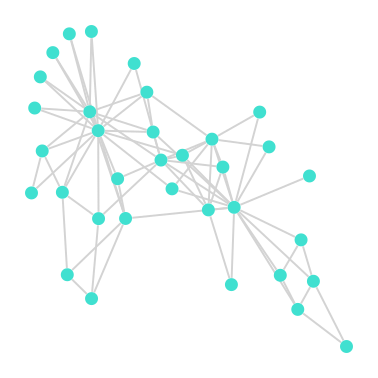
\includegraphics[width=0.45\textwidth]{../Imagenes/karate} 
	\end{center} 
	\vspace{-20pt} 
	\caption{Red de Karate.} 
	\vspace{-10pt}
	\label{fig:RedKarate}
\end{wrapfigure} 
En el mundo es posible encontrar diferentes tipos de redes con cierto significado, tales como la red de energética de un país, redes de amistades en una universidad o redes de acciones que cotizan en la bolsa de valores. Para poder representar estas redes y cualquier otro tipo de red conviene introducir el concepto de \textit{matriz de adyacencia.}
\newtheorem{defin1}{Definición}
\begin{defin1}
	Sea $A\in\mathcal{M}_n(\mathbb{R}) $. Se define la matriz de adyacencia tal que sus entradas son de la siguiente forma
	$$a_{ij}= 
	\begin{cases}
		1, \ \text{si $\exists$ un enlace entre el nodo $i$ y el nodo $j$.}\\
		0, \ \text{en otro caso}.
	\end{cases}$$
\end{defin1}
Para nuestros fines, la matriz de adyacencia nos indica la existencia o no de una interacción entre especies. Red dirigida y red no dirigida...


 
\end{document}